\chapter{Results of experiments with \carrp}
\label{app:cap}
\textit{This Appendix presents graphically a summary of individuals runs using \carrp. Figures show a \textit{box-plot} representation for different strategies and a bar representation for the percentage of winner solvers types.}
\vfill
\newpage

In Figure~\ref{boxplot:comm}, labels of the x-axis correspond to the following strategies:

\poslcaptiondesciption{
\begin{tabular}[t]{rl}
\textbf{NC}: & Non communication strategy \\
\textbf{A1-1}: & 100\% of communicating solvers performing the \commstr{} A \oneTone \\
\textbf{B1-1}: & 100\% of communicating solvers performing the \commstr{} B \oneTone \\
\textbf{A1-n}: & 100\% of communicating solvers performing the \commstr{} A \oneTn \\
\textbf{B1-n}: & 100\% of communicating solvers performing the \commstr{} B \oneTn \\
\textbf{50A1-1}: & 50\% of communicating solvers performing the \commstr{} A \oneTone \\ 
\textbf{50B1-1}: & 50\% of communicating solvers performing the \commstr{} B \oneTone \\
\textbf{50A1-n}: & 50\% of communicating solvers performing the \commstr{} A \oneTn \\
\textbf{50B1-n}: & 50\% of communicating solvers performing the \commstr{} B \oneTn \\
\end{tabular}
}

Figure~\ref{barplot:19} represents the percentage of winner solvers for each communication strategy, according to four different types:

\poslcaptiondesciption{
\begin{tabular}[t]{rl}
\receiver{Receiver}: & Receiver solver wining thanks to the received information \\
\sender{Sender}: & Sender solver \\
%\nonreceiver{Pasive receiver}: & Receiver solver wining without using the received information \\
\textbf{Non communicating}: & Non communicating solver \\
\end{tabular}
}

\begin{figure}[!h]
\centering
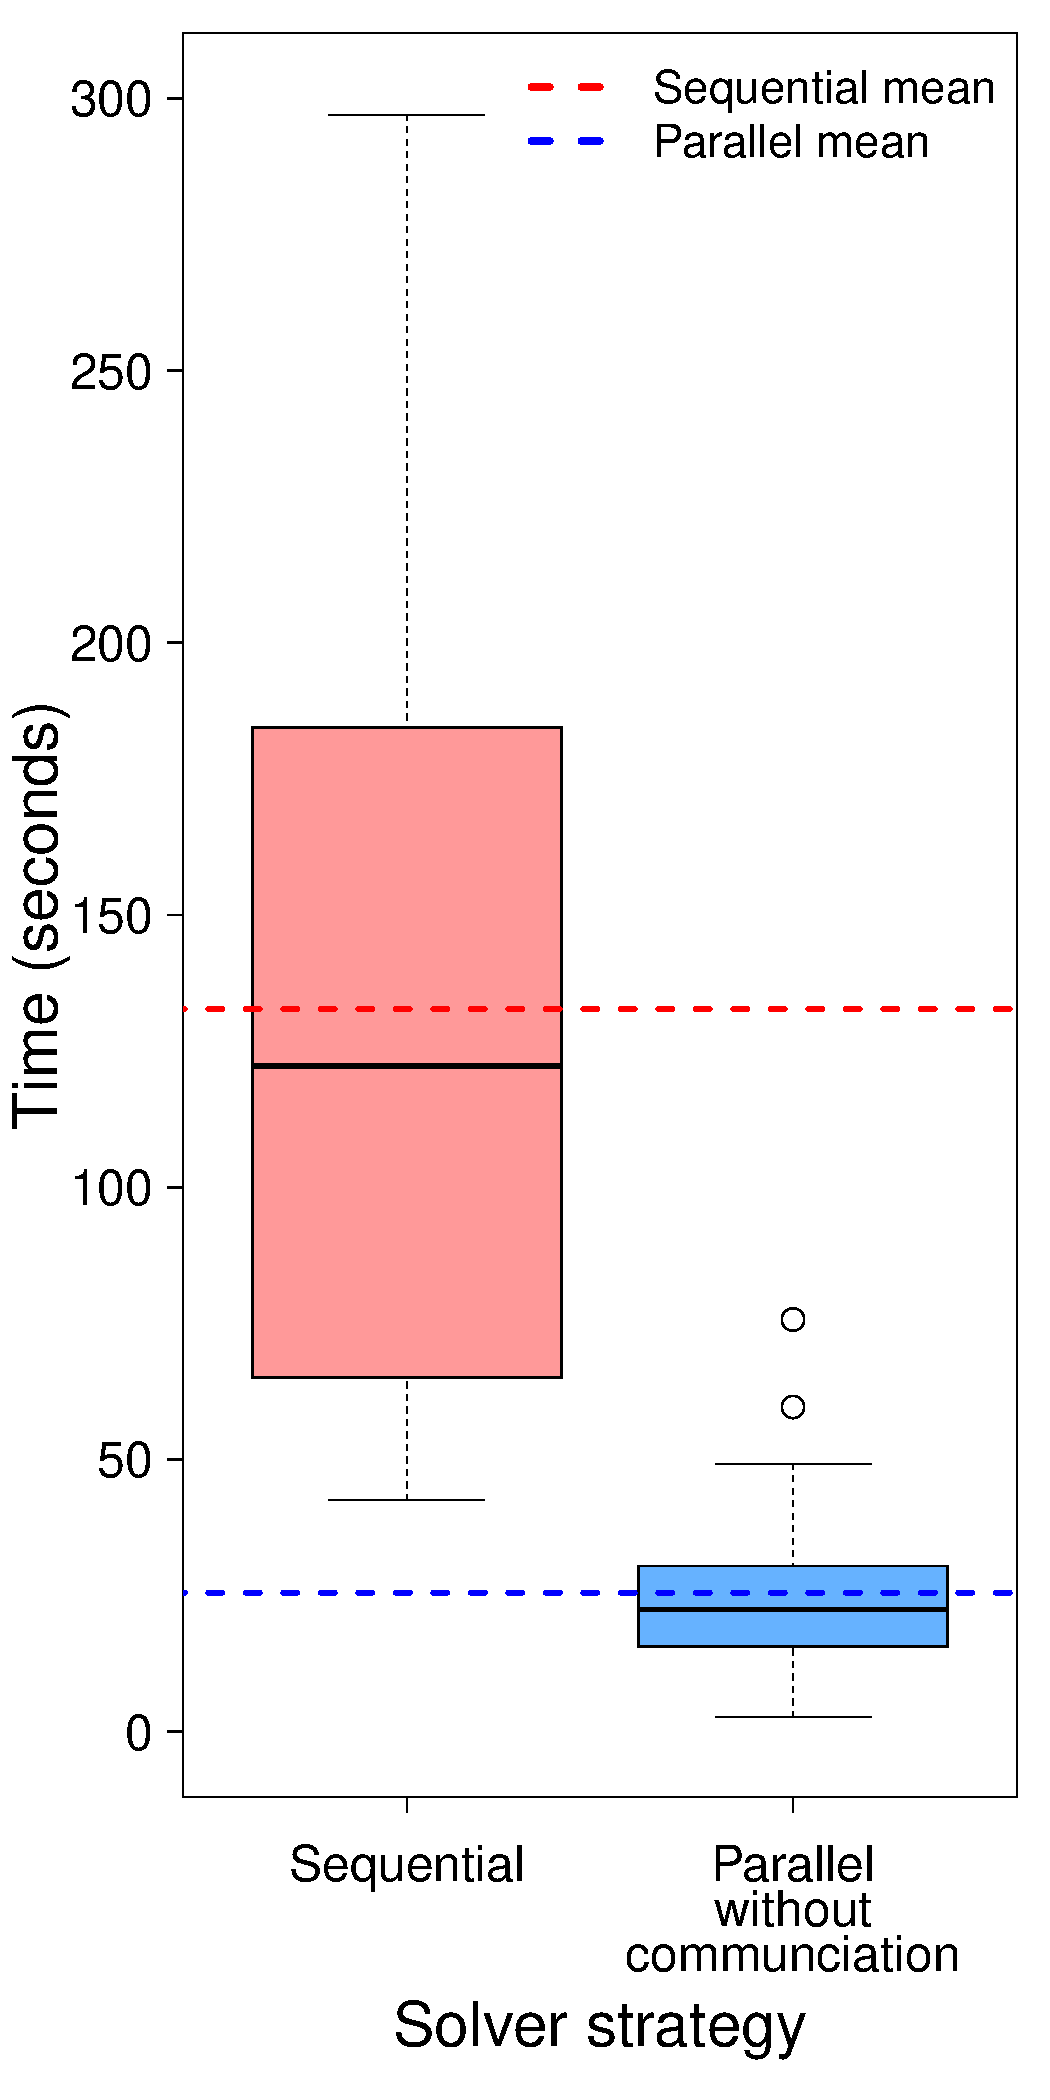
\includegraphics[width=0.3\textwidth]{c19_select_BP.pdf}
\caption{Comparison between sequential and parallel runs to solve \CARRP{} 19 using \posl}
\end{figure}

\begin{figure}[!h]
\centering
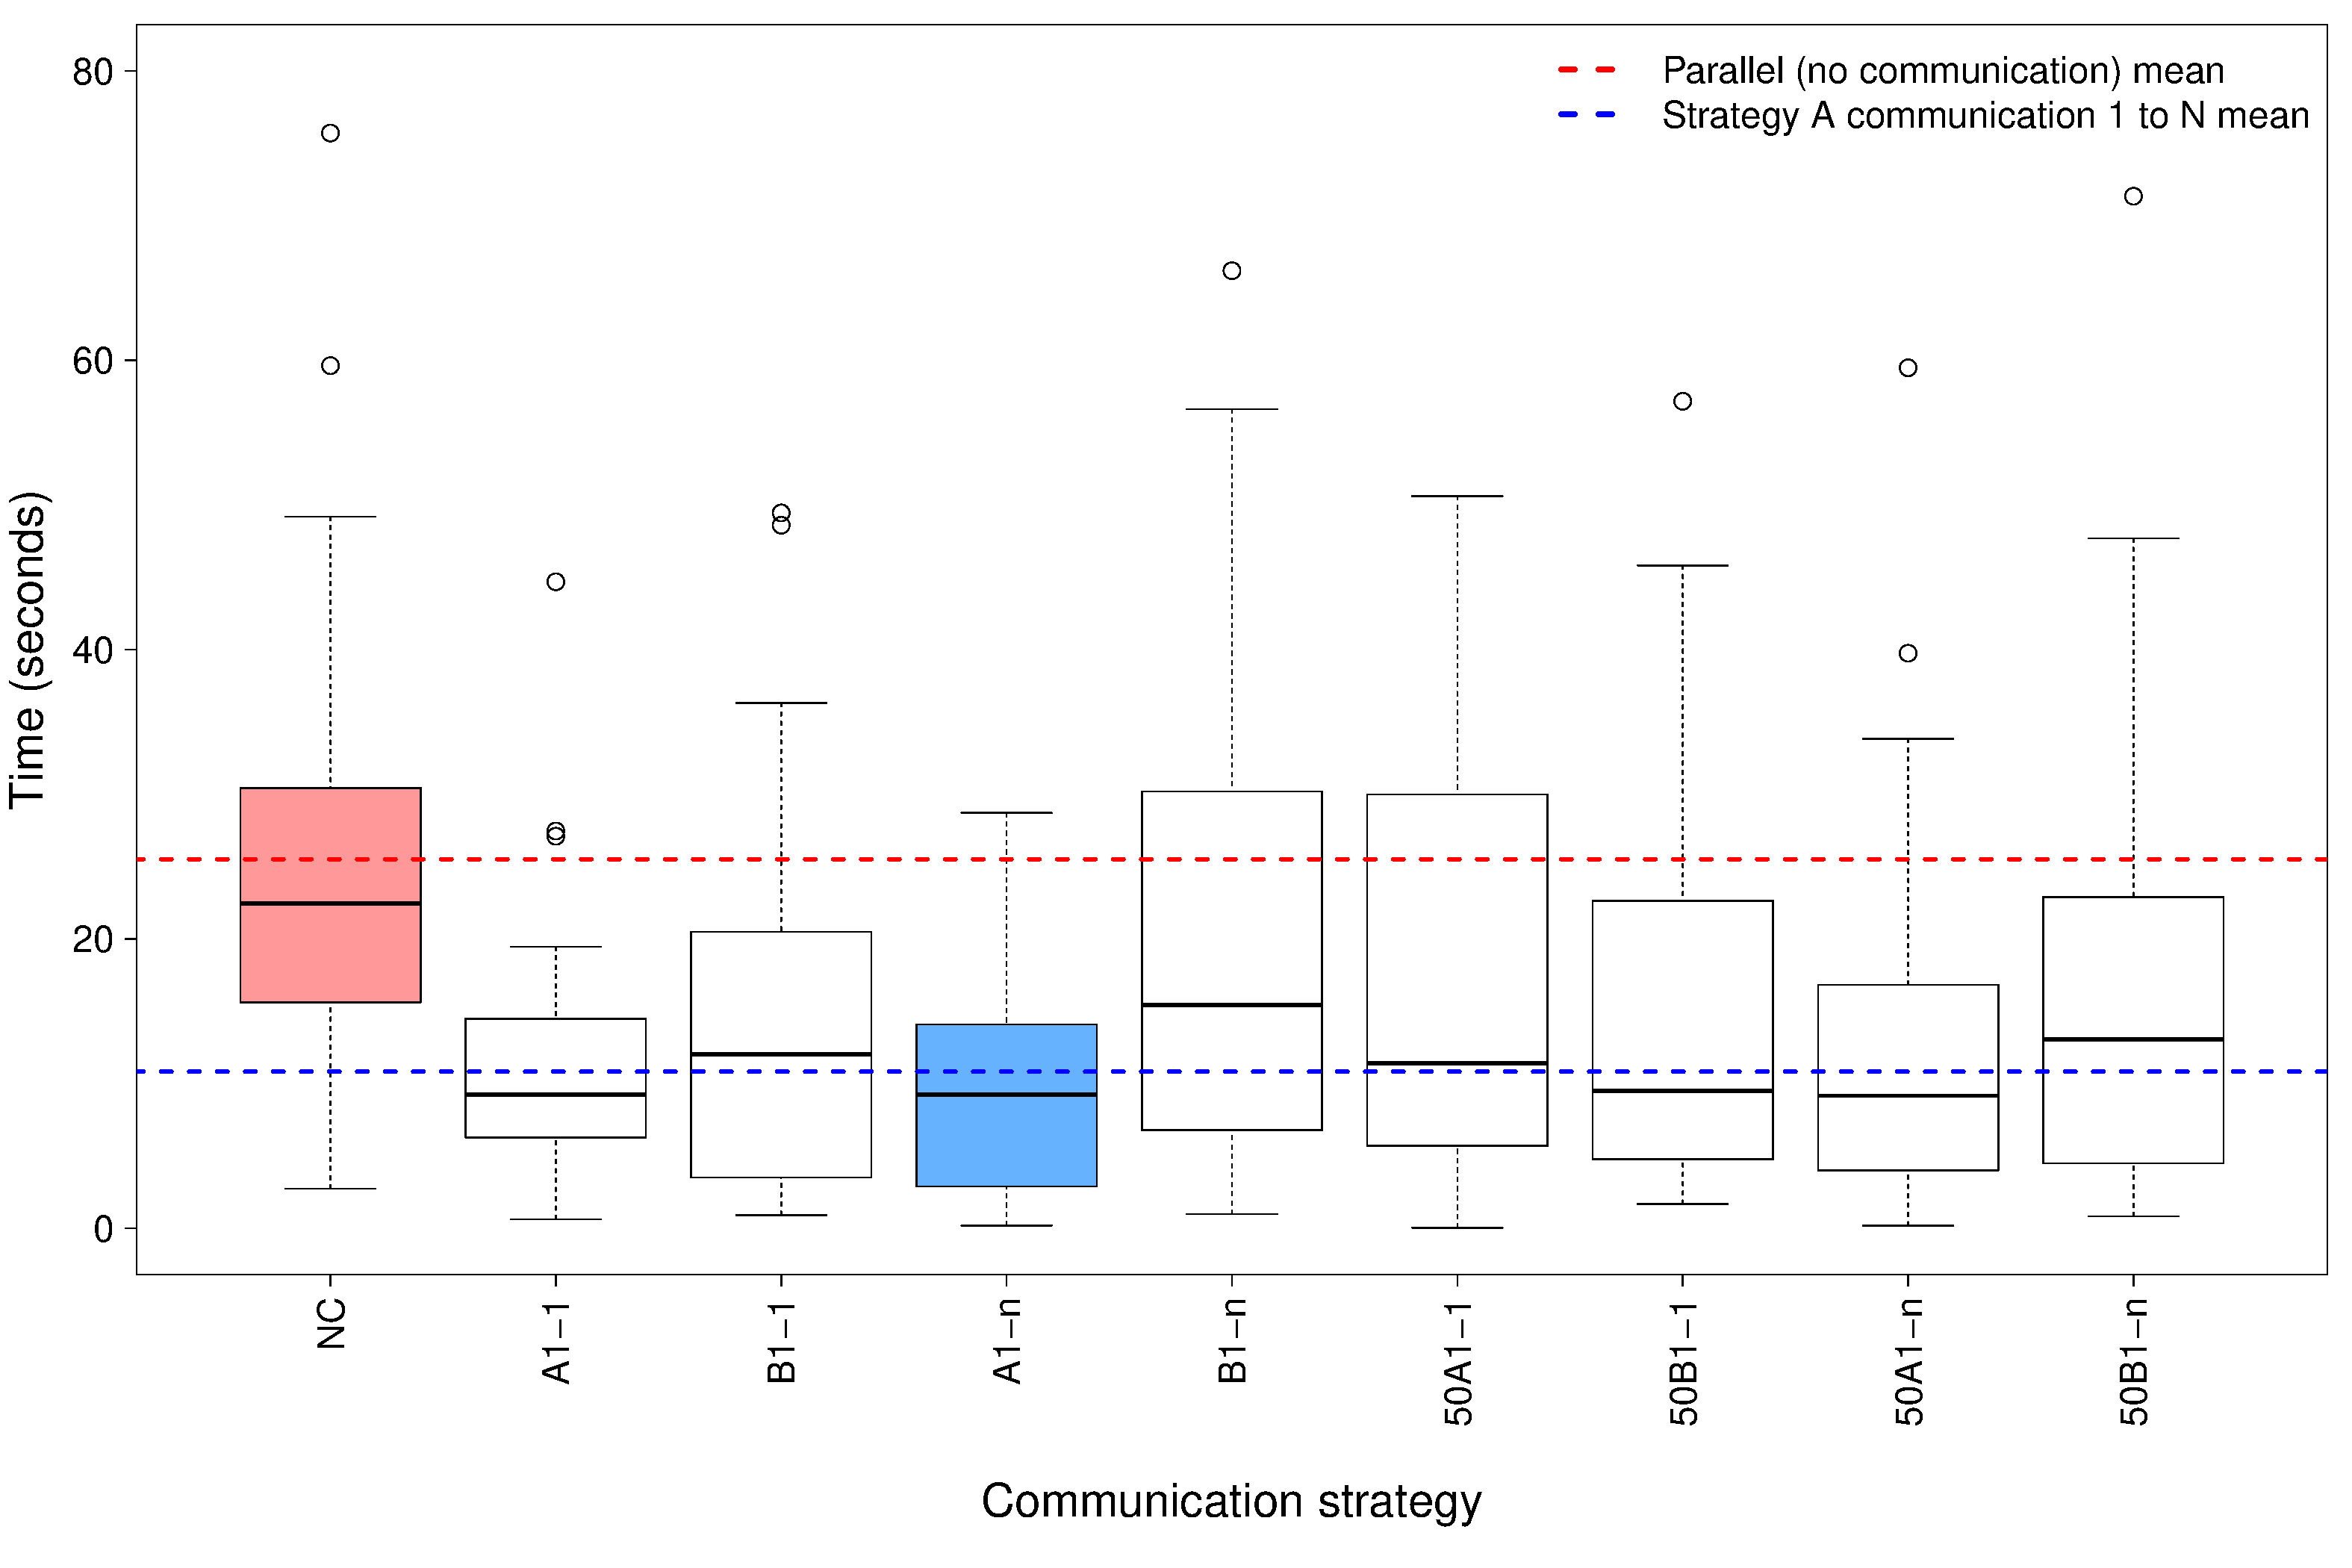
\includegraphics[width=0.8\textwidth]{c19_comm_BP.pdf}
\caption{Different communication strategies to solve \CARRP{} 19 using \posl}\label{boxplot:comm}
\end{figure}

\begin{figure}[!h]
\centering
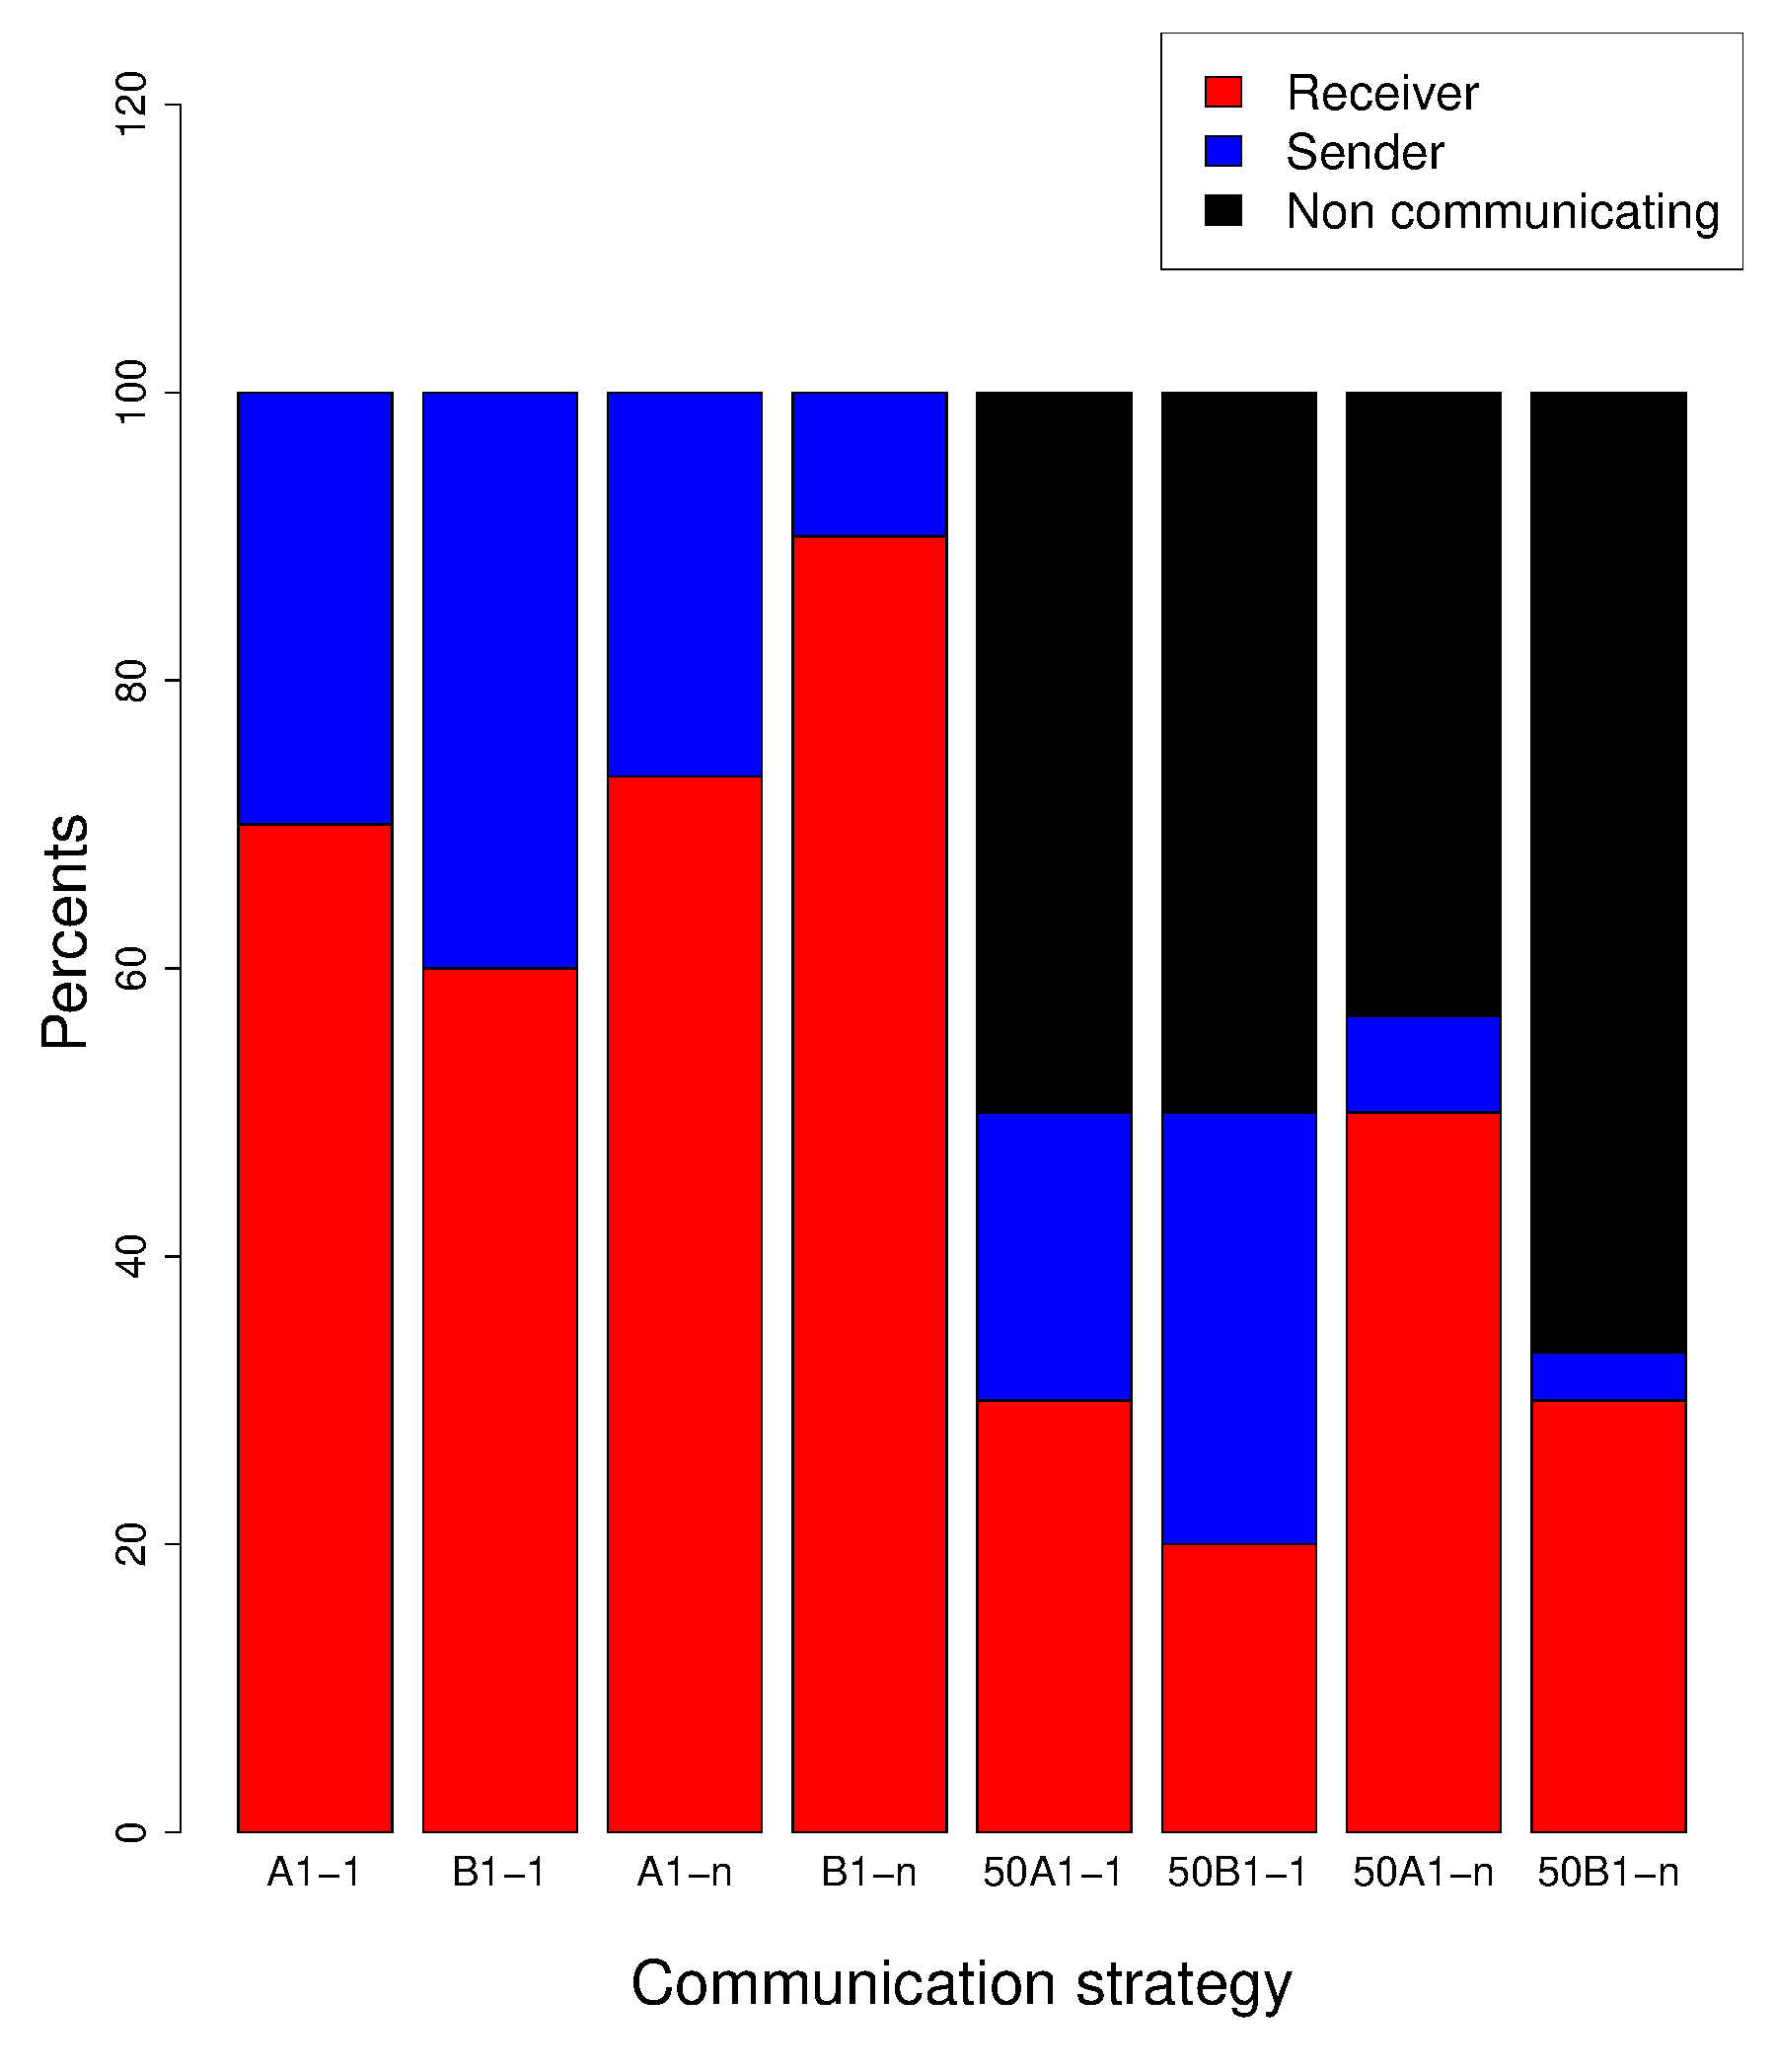
\includegraphics[width=0.6\textwidth]{c19_per_BP.pdf}
\caption{Solver proportion for each communication strategy to solve \CARRP{} 19 using \posl}\label{barplot:19}
\end{figure}